\begin{abstract}
A model can choose the right intervention by following an irrelevant numerical cue. It can also change its answer when the target population changes but reverse in the wrong direction. We introduce CF-TP1, a synthetic evaluation in which the same displayed rates admit two feasible assignments of randomized and historical evidence. Two target mixtures can require either a switch or an invariant decision. A matched scorecard names the governing table and specifies the arithmetic. In a prospective case study, one Qwen2.5-7B-Instruct Q4\_K\_M deployment completed 4,096 decisions on 128 independently sampled numerical families. On the prespecified transfer form, it answered both target variants correctly in 128/512 causal pairs and 146/512 arithmetic pairs. The family-standardized difference was $-3.52$ percentage points (approximate 95\% interval $-7.77$ to $+0.74$). The primary comparison was inconclusive. In prespecified diagnostics, the model activated in 995/1,024 causal decisions and correctly reversed in 3/256 required target switches. Arithmetic answers changed in 46/256 required switches and 45/256 invariant pairs. Directional scoring thus exposed a preference and unwarranted changes that aggregate accuracy obscured. The findings concern one deployment and two fixed forms. They support the instrument's diagnostic value while leaving causal-specific impairment and internal reasoning mechanisms unresolved.
\end{abstract}
\begin{IEEEkeywords}
causal inference, language model evaluation, target populations, behavioral testing, intervention decisions
\end{IEEEkeywords}

\section{Introduction}
Suppose two studies report the success of switching a setting on or off. One randomized the setting. In the other, operators chose it partly in response to an unrecorded risk. A model recommends switching on. Even if this recommendation is correct, two questions remain. Would it change if the other study had supplied the randomized evidence? Would it change in the right direction if the people who will receive the intervention had a different mix of risks?

We evaluate these questions as a proof-of-concept case study on one quantized 7B model. The empirical result tests whether the benchmark reveals distinct error patterns in that deployment; it cannot establish a general performance level across models.

An earlier prospective evidence-order study illustrates the problem. On conflict items from 96 fresh numerical families, a quantized model scored 175/192 with historical evidence first and 55/192 with randomized evidence first. Reversing the two blocks moved accuracy by 62.5 percentage points even though the evidence and correct action were identical. A subsequent audit found a rule that solved every prompt in either order. It takes the two printed on-minus-off differences, selects the one with smaller absolute magnitude and returns its sign. The rule never reads which study randomized treatment. Its success leaves the measured order effect intact, but it makes even a perfect score on this fixture ambiguous evidence of causal source use.

We therefore ask which changes in a recommendation can be attributed, at the level of observable behavior, to the information that determines the correct action. CF-TP1 varies two pieces of that information independently. The first is which of two tables reports randomized outcomes. The second is the proportion of a target population in each of two pretreatment strata. At a fixed source assignment, let $\delta_s$ be the trial's on-minus-off difference in success probability in stratum $s$, and let $w_k$ be the share of stratum 1 in target $k$. If the stratum effects carry over, treatment has no additional cost, and the objective is to maximize success, standardization gives the effect and decision \citep{transport,trial}
\begin{equation}
\tau_k = w_k\delta_1+(1-w_k)\delta_0,\qquad
a_k^\star=\mathbf{1}\{\tau_k>0\}.
\label{eq:target}
\end{equation}
When the two strata benefit from different actions, their relative sizes can determine which action to take. In the released example in Figure~\ref{fig:1}, increasing one stratum's share from 58\% to 83\% changes the preferred action from off to on when table L is randomized. With table R randomized, the same population shift calls for the opposite reversal. Both assignments are possible under an explicit data-generating model. Each prompt presents just one world and one target.

\begin{figure*}[t]\centering
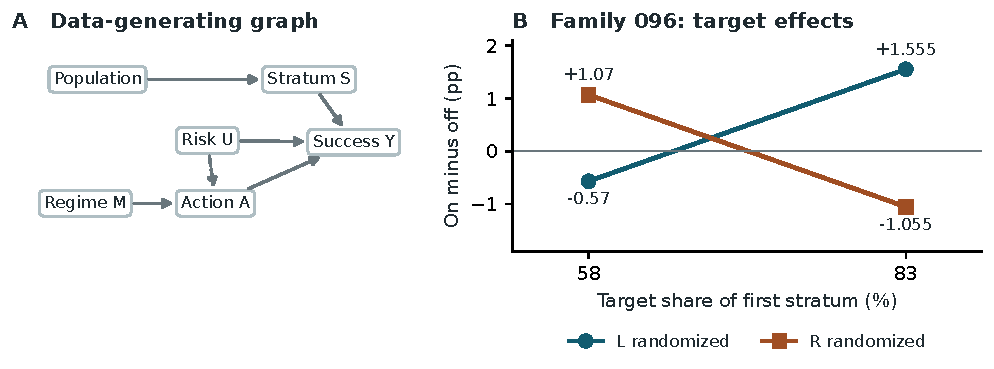
\includegraphics[width=.9\textwidth]{figures/fig1.pdf}
\caption{From study design to a target decision. The dashed risk-to-action edge operates in the historical study. The right panel gives the target effect in percentage points for family 096 under each feasible assignment. A positive effect favors switching on.}\label{fig:1}
\end{figure*}

The evaluator pairs responses after collection. At fixed wording, task, source order and governing table, let $\hat a_k$ denote the model's response for target $k$. A pair earns credit only when both decisions are valid and have the correct direction. Writing $I_k$ for the correctness of each member, we score
\begin{equation}
 I_k=\mathbf{1}\{\hat a_k\text{ is valid and }\hat a_k=a_k^\star\},
 \qquad F_{\mathrm{pair}}= I_0 I_1 .
 \label{eq:pair}
\end{equation}
Figure~\ref{fig:2} applies this rule to the same hypothetical answers across four designs. A model that says on then off can earn credit for a required reversal, reverse in the wrong direction, or change an answer that should have stayed fixed. Counting changes alone would score its behavior identically in all three cases.

\begin{figure*}[t]\centering
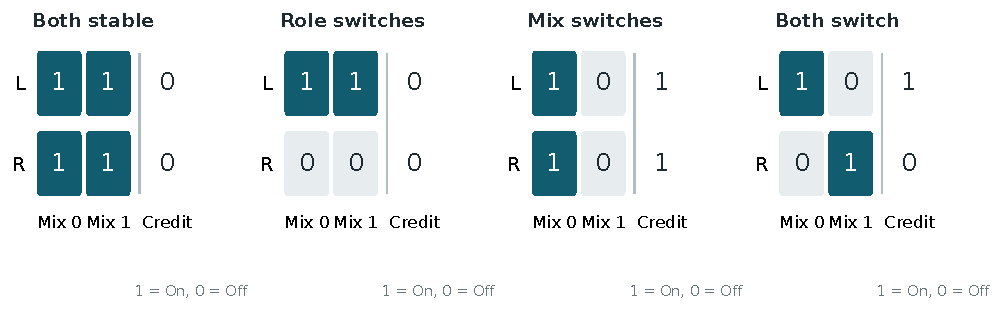
\includegraphics[width=.9\textwidth]{figures/fig2.pdf}
\caption{How the evaluator scores a change of answer. Each row gives the oracle actions at two target mixtures when L or R governs. The credit column scores the hypothetical responses on then off against that row. Each panel shows one sign pattern from the release. Its complement also occurs.}\label{fig:2}
\end{figure*}

A matched arithmetic prompt names the governing table and tells the model how to weight the rates. It uses the same numbers, target, answer order and scoring rule as its causal counterpart. The primary comparison averages the causal-minus-arithmetic fidelity difference within each numerical family, then across the eight design strata. Separate checks of source-role changes, physical reordering and action preference show where an aggregate score can mislead. The independent sampling unit is the numerical family. We verify each answer key by enumerating the underlying world and parsing the exact prompt. The single quantized 7B deployment supplies a proof-of-concept case study of the benchmark.

\section{Related work}
CLadder generates formal causal questions with computable answers across levels of the causal hierarchy \citep{cladder}. Broader behavioral studies of causal tasks also find that a language model's performance depends on how the task is posed \citep{causallm}. CausalFlip uses pairs of closely matched causal judgments with opposite answers \citep{flip}. EconCausal studies whether the sign of an economic effect transfers across empirical contexts \citep{econ}. CausalReasoningBenchmark scores the specification of an identification strategy separately from its numerical execution on real data \citep{crb}. In CF-TP1 the identifying assumptions are supplied, rates are exact, and the output is an action. The arithmetic comparator changes two parts of the instruction together. It permits a comparison of complete tasks, with less diagnostic resolution about intermediate steps than an explicit strategy specification.

Source interventions are also established. \emph{What Counts as Evidence?} manipulates epistemic cues to separate identification of cues from their influence on a judgment \citep{cue}. Contrast sets probe local decision boundaries, and CheckList formalizes invariance and directional expectations \citep{contrast,checklist}. Challenge sets can reveal that a heuristic and the intended rule produce the same predictions on an original test \citep{shortcut}. Position effects have been documented both for evidence within long contexts and for the ordering of answer alternatives \citep{middle,position}. Those studies motivate separate manipulations of source order and answer order here. Neither result predicts the direction of an effect on these short numerical prompts.

Studies of precision formats have directly compared compressed models on interventional and counterfactual questions \citep{compress}. An inference about compression requires a comparable reference deployment. Our final study fixes the model and format. Its contribution lies in examining what an observed action score can identify. The factorial structure also draws on psychological designs that cross cues and distinguish sensitivity from a tendency to respond in one direction \citep{jacoby,cni,sdt}. The observable crossover is useful even when the assumptions that would identify a latent process parameter are unavailable.

\section{Causal model and target decision}
Let $S$ denote a binary pretreatment stratum, $U$ an unobserved binary risk, $A$ a binary treatment, and $Y$ binary success. In the study population $S$ and $U$ are independent fair Bernoulli variables. In target $k$, $P_k(S=1)=w_k$ and $P_k(U=1\mid S)=1/2$. A trial assigns $A$ by an independent fair coin. In the historical regime, $P(A=1\mid S,U=u)=(1+2u)/4$. With an independent uniform error $E_Y$, the structural equation is $Y=\mathbf{1}\{E_Y<m_{SUA}\}$. Setting $A=a$ gives the potential outcome $Y(a)=\mathbf{1}\{E_Y<m_{SUa}\}$. Figure~\ref{fig:1} shows how the population and assignment regime enter the graph.

For a particular role assignment let $r_{sa}$ be the randomized rate of success in stratum $s$ under action $a$. Consistency, no interference, and within-trial randomization identify $\delta_s=r_{s1}-r_{s0}$ as the mean causal effect in that stratum. Given positive support for both strata and actions and transport of conditional mean effects, the law of total expectation yields equation~\eqref{eq:target} for $\tau_k=E_k[Y(1)-Y(0)]$.
This rule values success equally across strata and assigns no additional treatment cost. The construction makes the entire conditional response surface invariant across populations, a sufficient condition stronger than transport of the mean effect. The percentages represent population probabilities. Uncertainty in this study comes from sampling numerical families. Patient-level sampling error plays no role. Standardization and the assumptions licensing transport are established causal-inference methods \citep{transport,trial}.

\paragraph{Why the role swap is feasible.}
Write $h_{sa}$ for a displayed historical rate. At fixed $s,a$, put $r=r_{sa}$ and $h=h_{sa}$. The trial mixes $U=0,1$ equally. Historical assignment gives those two risk levels weights $(3/4,1/4)$ for $a=0$ and $(1/4,3/4)$ for $a=1$. Solving these two linear equations gives
\[
(m_{s0a},m_{s1a})=
\begin{cases}
(2h-r,\;3r-2h),&a=0,\\
(3r-2h,\;2h-r),&a=1.
\end{cases}
\]
The generator checks that every entry is strictly between zero and one, then repeats the construction with the roles exchanged. Thus identical displayed tables can arise in two distinct worlds. Within each world only the target mixture changes across the target pair. A source swap has a causal interpretation without an assumption that an actual observational study could be relabeled a trial.

\paragraph{Worked released family.}
In family 096, the off/on rates for the two strata in table L are $(51,54)$ and $(53,47.5)$ percent. The corresponding rates in R are $(52.5,50)$ and $(53.5,59.5)$. The first stratum's share rises from 0.58 to 0.83. With L randomized, equation~\eqref{eq:target} gives $0.58(3)+0.42(-5.5)=-0.570$ and $0.83(3)+0.17(-5.5)=+1.555$ percentage points (pp). The decision changes from off to on. With R randomized, the contrasts $(-2.5,+6)$ give $+1.070$ and $-1.055$ pp, reversing the two decisions. The majority stratum stays the same. An instructed arithmetic solver given the corresponding table obtains exactly the same four keys.

\section{Benchmark design and experimental setup}
The generator assigns 16 independent numerical draws to each combination of three binary factors. These specify whether changing target reverses the sign ($p$), whether changing source role reverses the sign ($g$), and the signed effect $b\in\{-1,1\}$ at the first corner. At role $r$ and target $k$, the required sign is $b(-1)^{gr+pk}$. Rejection sampling enforces this pattern under both feasible role worlds, a minimum absolute target effect of 0.50 pp and distinct source effect profiles. Both sources have opposing stratum effects. Target weights vary even within invariant pairs. Figure~\ref{fig:2} shows the four resulting families of comparisons.

\begin{table*}[t]\centering\caption{Design and conditions. Only numerical families are independent sampling units.}\label{tab:design}\small
\begin{tabularx}{\linewidth}{@{}lX@{}}\toprule
Factor & Levels and interpretation\\\midrule
Family sample & 128 independent slots in eight equal sign strata. Each slot fixes two tables, two target weights and four administration bits.\\
Form & Archive-compatible and transfer wording. Both were frozen and interleaved. Transfer was primary.\\
Task & Causal study interpretation or explicitly designated weighted scorecard. Both use the same numbers, target, alternatives and parser within a form.\\
Source order & L first or R first. Keys stay fixed. L and R are evaluator labels.\\
Governing role & L or R supplies randomized rates in the causal prompt and designated rates in the control.\\
Target & One of two mixtures per prompt. Under each role, the oracle determines whether the two keys agree.\\
Administration & Public source names, stratum names, answer-alternative order and within-table stratum order balanced across slots within sign stratum.\\
Schedule & $2^5=32$ stateless prompts per family. Four target pairs per family, task and form, from two orders and two roles.\\\bottomrule
\end{tabularx}\end{table*}

Figure~\ref{fig:prompts} reproduces one exact causal and arithmetic prompt pair from released family 096. The causal prompt describes random assignment, selection by operators and transport of stratum effects. The control uses the same data as a scorecard, names the governing table, and instructs the model to weight and add. It removes the need to recognize study provenance and to elicit the standardization procedure. Both tasks still require reading a table, weighting values, comparing scores, mapping the result to an action and returning it in the specified format. Neither context contains a worked answer. An enumerator computes each world's marginal rates and intervention scores. A separate parser computes scores from the rendered public text. Their exact rational scores and actions agree throughout. Independent \emph{implementation} is documented. Independent human certification of the transfer form before inference remains unverified.

\begin{figure*}[t]
\centering
\begin{minipage}[t]{.48\textwidth}\centering\textbf{Causal decision prompt}\par
\lstinputlisting{data/prompt-family096-causal.txt}
\end{minipage}\hfill
\begin{minipage}[t]{.48\textwidth}\centering\textbf{Matched arithmetic prompt}\par
\lstinputlisting{data/prompt-family096-arithmetic.txt}
\end{minipage}
\caption{Exact user messages from the transfer form for released family 096, first target, source A governing, source A displayed first. Both calls also used the same system message, ``You are completing a decision exercise. Follow the requested response format.'' The two input files are extracted verbatim from the frozen task file by task ID.}
\label{fig:prompts}
\end{figure*}

\paragraph{Deployment and freeze.}
One Qwen2.5-7B-Instruct GGUF Q4\_K\_M deployment received 4,096 fresh-context requests. The llama.cpp server ran on x86-64 CPU with eight threads, zero GPU layers, one slot, a 2,048-token context, and F16 key/value cache. Temperature was zero, sampling seed 20261126, and completion budget 48 tokens. Prompt caching and streaming were disabled. The fixture used master seed 290431 and the interleaved schedule used seed 290432. Frozen tokenizer counts include the chat template overhead. Model and server digests appear in the supplement. The journal binds every request to the production manifest. The pre-inference protocol and clarification are available in the repository. A third-party registration identifier is unavailable. The clarification retained literal failures for constant-output rivals and specified how to score them. Release-time reconstruction of the analysis followed collection.

\paragraph{Endpoint and uncertainty.}
A normal-stop completion had to contain exactly one JSON object with the single integer field \texttt{activate} equal to 0 or 1. Invalid answers score zero. At fixed family, form, task, source order and role, target-pair fidelity is the product in equation~\eqref{eq:pair}. For each transfer family $i$, let $D_i$ be causal fidelity averaged over its four pairs minus the analogous arithmetic mean. The prespecified estimate averages the eight within-stratum means of $D_i$ with equal weight. We report its approximate 95\% Welch--Satterthwaite interval and a conservative bounded interval. Independent units are the 128 family draws. The fixed prompts, repeated roles and two forms do not add sampling units. Switch, invariance, direction, order, validity and form diagnostics are descriptive. The supplement gives the variance estimator, missingness convention and calibration results.

\section{Results}
\paragraph{Prespecified primary comparison.}
On the transfer form, causal target-pair fidelity was 128/512 (25.00\%) and arithmetic fidelity was 146/512 (28.52\%). The family-standardized causal-minus-arithmetic contrast was -3.52 pp (SE 2.1324 pp, Welch df 67.53). The approximate 95\% interval ran from -7.77 to +0.74 pp. The bounded interval ran from -27.5 to +20.5 pp (Fig.~\ref{fig:3}). The primary comparison is inconclusive about a difference. An equivalence margin was never specified. All 4,096 scheduled responses were present and strict-valid, so complete-case and scheduled-denominator scores coincide.
\fplot{3}{Transfer-form fidelity and its paired contrast. Panel A shows descriptive 95\% family-stratified approximate intervals for each task, added for presentation. Panel B shows the two prespecified intervals for the causal-minus-arithmetic contrast. Its uncertainty uses within-family differences.}{1}

\paragraph{Switches, invariance and order.}
Only 8/256 causal target pairs changed action when a reversal was required. Three reversals had the correct orientation and five reversed in the wrong direction. On invariant target pairs the model stayed with its initial action in 249/256 cases, but both actions were correct in only 125/256. Arithmetic produced more changes. Their frequencies were almost identical when the target required a switch (46/256) and when it required invariance (45/256). Of the 46 required-pair changes, 27 had the correct orientation. Figure~\ref{fig:4} distinguishes the resulting errors. Table~\ref{tab:outcomes} applies the same scoring to changes in governing source and to physical reorderings.
\fplot{4}{Distribution of correctly answered members per transfer-form target pair. Of the 256 required causal reversals, three have both members correct, 248 have one, and five have neither. The same number of correct members can represent different behaviors across panels because the oracle changes only in panel A.}{1}

\begin{table*}[t]\centering\small\caption{Transfer-form outcomes. The two right-hand columns count changed actions irrespective of direction. A change under physical reordering is always unwarranted.}\label{tab:outcomes}
\begin{tabular}{@{}lrrrr@{}}\toprule
\multicolumn{5}{@{}l}{\textbf{Panel A: Paired consistency}}\\
 &\multicolumn{2}{c}{Both correct}&\multicolumn{2}{c}{Changed action}\\
Pair type & Causal & Arithmetic & Causal & Arithmetic\\\midrule
Target (primary) &128/512&146/512&15/512&91/512\\
\quad Switch &3/256&27/256&8/256&46/256\\
\quad Invariant &125/256&119/256&7/256&45/256\\
Source role, switch &10/256&34/256&19/256&65/256\\
Source role, invariant &123/256&123/256&8/256&42/256\\
Physical order, invariant &241/512&187/512&29/512&173/512\\\midrule
\multicolumn{5}{@{}l}{\textbf{Panel B: Directional and aggregate outcomes}}\\
&\multicolumn{2}{c}{Causal}&\multicolumn{2}{c}{Arithmetic}\\
Correct when off required &\multicolumn{2}{c}{14/512}&\multicolumn{2}{c}{231/512}\\
Correct when on required &\multicolumn{2}{c}{497/512}&\multicolumn{2}{c}{316/512}\\
Activated &\multicolumn{2}{c}{995/1,024}&\multicolumn{2}{c}{597/1,024}\\
Scheduled row accuracy &\multicolumn{2}{c}{511/1,024}&\multicolumn{2}{c}{547/1,024}\\\bottomrule
\end{tabular}\end{table*}

\paragraph{Action direction, form and validity.}
The causal model responses favored activation under both oracle directions. Arithmetic responses were more distributed across actions. The counts in Table~\ref{tab:outcomes} come from the raw journal joined to the frozen keys. The archive-compatible form yielded 128/512 both-correct target pairs for each task, giving a zero contrast. The transfer-minus-archive difference in contrasts was therefore -3.52 pp. The two fixed wordings constrain interpretation of this comparison. Physical source order was crossed within family. Displayed answer order was balanced \emph{between} slots. In an additional descriptive breakdown, causal row accuracy was 256/512 with off listed first and 255/512 with on listed first. Arithmetic accuracy was 273/512 and 274/512 respectively. This breakdown cannot identify within-family susceptibility to answer order.

\paragraph{Deterministic comparisons.}
Always activating gets half the individual keys right, misses every switch pair, and solves half the invariant pairs. It therefore attains 25\% target-pair fidelity on this balanced suite, exactly the observed causal aggregate. The model did depart from the constant policy, including three correct target reversals. Equality of two aggregate scores cannot establish equality of policies. Table~\ref{tab:policies} illustrates the different signatures of rules fixed before inference. A source-blind rule must give the same answer after a pure role change. In the half of families with required role switches it can get at most half of the individual keys right, giving an overall item ceiling of 75\%. Target-blind rules analogously cannot solve a required target switch pair. The bounds apply to specified invariances of the rule. A solver that extracts the correct role lexically and then performs exact arithmetic is admissible.
\begin{table*}[t]\centering\small\caption{Deterministic fixture checks across both tasks and forms. Entries are numbers correct, with denominators in the header. Switch columns require both members correct. The stored first tie convention is shown.}\label{tab:policies}
\begin{tabular}{@{}lrrr@{}}\toprule
Policy & Items / 4,096 & Target switch / 1,024 & Role switch / 1,024\\\midrule
Always on &2,048&0&0\\
First table, exact weighting &3,072&768&0\\
Smaller absolute weighted effect &3,072&600&0\\
Governing table, equal weights &2,656&0&576\\
Governing table, majority stratum &3,072&0&768\\
Exact weighted contribution comparison &4,096&1,024&1,024\\\bottomrule
\end{tabular}\end{table*}

\paragraph{Separate prospective evidence-order study.}
On Qwen2.5-7B-Instruct Q4\_K\_M conflict items, historical-first accuracy was 175/192 versus 55/192 for randomized-first. The prespecified mean within-family difference was $+62.5$ pp (95\% family $t$ interval $+56.6$ to $+68.4$ pp, $t_{95}=21.10$, two-sided $p=1.24\times10^{-37}$). A family percentile bootstrap gave $+56.8$ to $+68.2$ pp. All 768 answers per format were strict-valid. The corresponding descriptive F16 counts were 109/192 and 76/192. On aligned Q4 items the order change instead moved accuracy from 192/192 randomized-first to 105/192 historical-first. The ordering therefore affected more than the resolution of direct disagreement.

A retrospective test parses only the two printed off/on gaps and chooses the sign of the smaller absolute gap. It matches 768/768 scheduled keys, including 384/384 conflict keys across both orders. Figure~\ref{fig:5} explains why it succeeds. Every trial gap is smaller than every historical gap in this particular fixture. This is a constructive counterexample to interpreting accuracy as proof of provenance use. It supplies no evidence that the model implemented that particular heuristic. These families and effects are excluded from the main study estimate.
\fplot{5}{Separate prospective evidence-order study. Panel A shows the measured order crossover on conflict prompts. Panel B shows one conflict example per family; magnitudes are constant across the two orders. Every point lies above equality. On this fixture, selecting the smaller absolute gap recovers the randomized contrast without reading the source label.}{1}

\section{Discussion}
A binary action can conceal two distinct errors. A model that responds off then on has recognized a target difference only in a weak behavioral sense. When the oracle requires on then off, both decisions are wrong. Conversely, a model that always activates can appear stable across nearly all invariant pairs, although it is correct only for the subset whose two keys are on. The joint distribution of zero, one and two correct members, stratified by whether a switch was required, distinguishes these possibilities. Single-item accuracy, agreement across prompts and the overall fraction of changed answers each discard part of this distribution.

The methodological gain over the earlier evidence-order study is that the final instrument breaks an explicit observational ambiguity. The two governing assignments can yield identical printed rates and opposite keys. A rule reading rates alone then cannot solve both. Independently, a single source's two opposite stratum effects can change their weighted sign as the target changes, so naming the trial alone cannot solve both target decisions. Invariant examples make an unconditional switch rule fail as well. These checks exclude specified shortcuts on designed contrasts while preserving legitimate numerical solutions. Table~\ref{tab:prior} places that combination in context.

\begin{table*}[t]\centering\small\caption{Comparison by the information varied and the object scored. Entries describe the cited task, without implying an exhaustive inventory of its capabilities.}\label{tab:prior}
\begin{tabularx}{\linewidth}{@{}>{\raggedright\arraybackslash}p{.28\linewidth}>{\raggedright\arraybackslash}X>{\raggedright\arraybackslash}X@{}}\toprule
Instrument & What changes & What the evaluation resolves\\\midrule
CLadder \citep{cladder} & Graph, causal query and formal data-generating instance & Correctness on questions with formal ground truth across causal levels\\
CausalFlip \citep{flip} & Causal query within closely matched event triples & Paired judgments when semantic similarity survives a label change\\
EconCausal \citep{econ} & Empirical economic context & Directional transfer across economically meaningful settings\\
CausalReasoning\-Benchmark \citep{crb} & Real research design and data & Identification specification and numerical estimate scored separately\\
What Counts as Evidence? \citep{cue} & Source, timing and presentation cues & Cue recognition, influence and competition\\
CF-TP1 & Feasible provenance assignment, target mix and display order & Direction-correct switches and invariances with exactly matched scorecards\\\bottomrule
\end{tabularx}\end{table*}

Earlier development studies found that a model could compute a numerical effect or identify the governing source yet still choose the wrong action. They also exposed sensitivity to answer mappings, position and response validity. These findings motivated the matched arithmetic control and the paired action endpoint. The complete development history and its inferential status appear in the supplement.

\paragraph{Limitations.}
The primary comparison covers a single quantized deployment. The main study has no F16 arm, and the earlier evidence-order study addresses another task. Synthetic rate tables provide exact keys at the cost of excluding trial sampling uncertainty, model misspecification and uncertain transport assumptions. The generator permits symmetric switch patterns across both levels of the other factor and deliberately excludes near-zero ties. Decisions in settings with treatment costs, asymmetric utility, continuous actions or incomplete identification require a different oracle. Two fixed English forms do not sample a population of phrasings. Their reading loads differ, and the arithmetic control makes source selection and weighting explicit together. Its own low paired fidelity and the interval crossing zero limit causal-specific attribution. No response trace identifies an internal causal algorithm, and the enumerated rival policies cannot exhaust all possible shortcuts. Transfer to other checkpoints, domains or tool-using systems remains open.

The frozen protocol documents computational checks, while independent human qualification of the transfer wording was not established before inference. The supplement records the provenance and later verification in detail.

\section{Conclusion}
CF-TP1 turns a correct intervention recommendation into a stronger test by asking which matched changes should reverse that recommendation and which should preserve it. In a completed deployment, causal and arithmetic paired fidelity differed by an imprecisely estimated 3.52 points in the arithmetic direction. Directional scoring exposed a near-constant causal action preference and frequent arithmetic changes without a corresponding change in the correct decision. The reusable contribution is the feasible paired construction, its public-text oracle, and a scoring procedure that makes those observations distinguishable.

\section*{Data, code and declarations}
The frozen fixture, responses, analyses and offline reproduction instructions are available in the \href{https://github.com/mutasim-rehman/project-causalfade/releases/tag/cohort-029-v1.0.0}{public release archive} (scientific commit \texttt{76206c2}). The scoped software license is MIT and the designated numerical fixture and analyses are CC BY 4.0. The exact transfer prompts in Fig.~\ref{fig:prompts} are archived for reproducibility under contributor-controlled rights. Permission to republish those exact words must be confirmed before journal submission.

The study uses synthetic populations and recorded model outputs and received no funding. OpenAI Codex assisted with manuscript drafting, computational checking, figures and compilation; the transfer-form author reported Claude assistance in drafting prompt wording.
